\subsection{Unraveling Total Radiated Power: Gains \& Losses Explained!}

\begin{tcolorbox}[colback=gray!10, colframe=black, title=E9A03] What term describing total radiated power takes into account all gains and losses?
\begin{enumerate}[label=\Alph*.]
    \item Power factor
    \item Half-power bandwidth
    \item \textbf{Effective radiated power}
    \item Apparent power
\end{enumerate} \end{tcolorbox}

\subsubsection{Elaboration on Related Concepts}

In the field of radio communications and electronics, understanding the total radiated power of an antenna system is crucial. The term that accurately describes the total radiated power while considering all gains and losses in the system is known as \textbf{Effective Radiated Power (ERP):}.

\subsubsection{Key Concepts}

1. \textbf{Gain:}: Antenna gain measures how well the antenna converts input power into radio waves focused in a particular direction. It is expressed in decibels (dB).
  
2. \textbf{Losses:}: Various factors can lead to power losses, including:
   - Cable losses: Losses that occur in the transmission lines and connectors.
   - Resistive losses: Losses due to the resistance of the materials used in the antenna system.
   - Environmental losses: Reflections and absorptions from the surrounding environment.

3. \textbf{Effective Radiated Power (ERP):}: This is the actual power radiated by an antenna, taking into account its gain and any losses through the system. It can be calculated as:
   \[
   \text{ERP} = P_t + G_a - L
   \]
   where \( P_t \) is the transmitter power in dBm, \( G_a \) is the antenna gain in dBi, and \( L \) is the losses in dB.

\subsubsection{Calculation Example}

Suppose we have the following values:
- Transmitter Power, \( P_t = 50 \, \text{W} \) (which is \( 10 \cdot \log_{10}(50) \approx 17 \, \text{dBm} \))
- Antenna Gain, \( G_a = 6 \, \text{dBi} \)
- Losses, \( L = 3 \, \text{dB} \)

Using the formula:
\[
\text{ERP} = P_t + G_a - L
\]
We substitute the values:
\[
\text{ERP} = 17 \, \text{dBm} + 6 \, \text{dBi} - 3 \, \text{dB} = 20 \, \text{dBm}
\]

Thus, the effective radiated power is \( 20 \, \text{dBm} \).

\subsubsection{Diagram of Antenna System}

\begin{center}
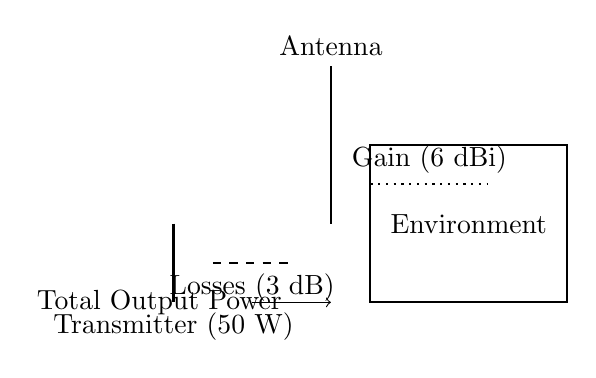
\begin{tikzpicture}
    % Draw the antenna
    \draw[thick] (0,0) -- (0,2) node[above] {Antenna};
    
    % Draw the transmitter
    \draw[thick] (-2,0) -- (-2,-1) node[below] {Transmitter (50 W)};
    
    % Draw the losses
    \draw[thick,dashed] (-1.5,-0.5) -- (-0.5,-0.5) node[midway,below] {Losses (3 dB)};
    
    % Draw the environment
    \draw[thick] (0.5,-1) rectangle (3,1) node[midway] {Environment};
    
    % Draw the gains
    \draw[thick,dotted] (0.5,0.5) -- (2,0.5) node[midway,above] {Gain (6 dBi)};
    
    % Connect parts
    \draw[->] (-1,-1) -- (0,-1) node[midway,left] {Total Output Power};
\end{tikzpicture}
\end{center}

By understanding Effective Radiated Power, one can optimize antenna designs and improve communication system efficiencies.
